\documentclass[10pt, compress]{beamer}

\usetheme{m}

\usepackage{booktabs}
\usepackage[scale=2]{ccicons}

\usepgfplotslibrary{dateplot}
\usepackage{tikz}
\usetikzlibrary{shapes,shadows,calc}
\usepgflibrary{arrows}
\usetikzlibrary{fit}

\title{ceph workshop}
\subtitle{GridKA School 2015}
\date{\today}
\author{Diana Gudu}
\institute[KIT]{Karlsruhe Institute of Technology}

\begin{document}

\maketitle

\begin{frame}[fragile]
  \frametitle{evolution of storage}
    \begin{center}
        \tikzset{
  sshadow/.style={opacity=.25, shadow xshift=0.05, shadow yshift=-0.06},
}

%-----TBoxes
%-----#1 height, #2 width, #3 anchor for the label, #4 name of the node, #5
%-----coordinate, #6 label
\def\tboxr[#1,#2,#3,#4,#5]#6{%
  \node[draw, drop shadow={opacity=.35}, minimum height=#1, minimum width=#2, %
  inner color=black!2, outer color=black!2, color=mDarkTeal] (#4) at #5 {}; %
  \node[anchor=#3,inner sep=2pt] at (#4.#3) {#6}; %
}

%-----#1 name of the node, #2 coordinate, #3 label
\def\entity[#1,#2]#3;{
  \node[draw,drop shadow={opacity=.4,shadow xshift=0.04, shadow
    yshift=-0.04},color=mDarkTeal,fill=black!2,rounded corners=3] (#1) at #2 {#3};
}
\def\ragent[#1,#2]#3;{
  \node[draw,drop shadow={opacity=.4,shadow xshift=0.04, shadow
    yshift=-0.04},color=mDarkTeal,fill=mLightBrown!20,rounded corners=3] (#1) at #2 {#3};
}

%-----#1 from node, #2 to node, #3 specification of a node (label), #4
%-----dashed, or other parameters for draw
\def\isaedge[#1,#2,#3,#4];{ 
  \draw[to-to,color=mDarkTeal,#4,fill=mDarkTeal] (#1) -- #3
  (#2);  
}

%-----ABoxes
%-----#1 height, #2 width, #3 aspect, #4 name of the node, #5
%-----coordinate, #6 label
\def\aboxr[#1,#2,#3,#4,#5]#6{%
  \node[draw, cylinder, alias=cyl, shape border rotate=90, aspect=#3, %
  minimum height=#1, minimum width=#2, outer sep=-0.5\pgflinewidth, %
  color=orange!20, left color=mLightBrown, right color=mLightBrown
  ] (#4) at #5 {};%
  \node at #5 {#6};%
  \fill [mLightBrown] let \p1 = ($(cyl.before top)!0.5!(cyl.after top)$), \p2 =
  (cyl.top), \p3 = (cyl.before top), \n1={veclen(\x3-\x1,\y3-\y1)},
  \n2={veclen(\x2-\x1,\y2-\y1)} in (\p1) ellipse (\n1 and \n2); }

\begin{tikzpicture}[
    mnode/.style={circle,draw=black,fill=black,inner sep=0pt,minimum size=0.5pt},
    %scale=0.7
    ]
\small

    \only<1-4>{
    \ragent[cl1,(0,5)]{\tiny Human};
    \entity[pc1,(0,2)] {\tiny Computer};
    \aboxr[10,20,1.2,d1,(0,0)]{\tiny Disk};
    \isaedge[cl1,pc1,,];
    \isaedge[pc1,d1,,];
    }

    \only<2-4>{
    \aboxr[10,20,1.2,d2,(1,0)]{\tiny Disk};
    \aboxr[10,20,1.2,d3,(2,0)]{\tiny Disk};
    \aboxr[10,20,1.2,d4,(-1,0)]{\tiny Disk};
    \aboxr[10,20,1.2,d5,(-2,0)]{\tiny Disk};
    \isaedge[pc1,d2,,];
    \isaedge[pc1,d3,,];
    \isaedge[pc1,d4,,];
    \isaedge[pc1,d5,,];
    \ragent[cl2,(1,5)]{\tiny Human};
    \ragent[cl3,(-1,5)]{\tiny Human};
    \isaedge[cl2,pc1,,];
    \isaedge[cl3,pc1,,];
    }
    
    \only<3-4>{
    \ragent[cl4,(2,4)]{\tiny Human};
    \ragent[cl5,(-2,4)]{\tiny Human};
    \ragent[cl6,(3,4)]{\tiny Human};
    \ragent[cl7,(-3,4)]{\tiny Human};
    \ragent[cl8,(-2,3)]{\tiny Human};
    \ragent[cl9,(2,3)]{\tiny Human};
    \ragent[cl10,(2,5)]{\tiny Human};
    \ragent[cl11,(0,4)]{\tiny Human};
    \ragent[cl12,(-1,4)]{\tiny Human};
    \ragent[cl13,(1,4)]{\tiny Human};
    \ragent[cl14,(-2,5)]{\tiny Human};
    \isaedge[cl4,pc1,,];
    \isaedge[cl5,pc1,,];
    \isaedge[cl6,pc1,,];
    \isaedge[cl7,pc1,,];
    \isaedge[cl8,pc1,,];
    \isaedge[cl9,pc1,,];
    \isaedge[cl10,pc1,,];
    \isaedge[cl11,pc1,,];
    \isaedge[cl12,pc1,,];
    \isaedge[cl13,pc1,,];
    \isaedge[cl14,pc1,,];
    }

    \only<4>{
    \tboxr[25,60,center,pc1,(0,2)]{\tiny Big Expensive Computer};
    }

    \only<5->{
    \ragent[cl1,(0.1,3)]{\tiny Human};
    \ragent[cl2,(1.1,3)]{\tiny Human};
    \ragent[cl3,(-1.1,3)]{\tiny Human};
    }

    \only<5>{
    \entity[pc1,(0,0.6)] {\tiny Computer};
    \entity[pc2,(1,0.6)] {\tiny Computer};
    \entity[pc3,(2,0.6)] {\tiny Computer};
    \entity[pc4,(-1,0.6)] {\tiny Computer};
    \entity[pc5,(-2,0.6)] {\tiny Computer};
    \aboxr[10,20,1.2,d1,(0,0)]{\tiny Disk};
    \aboxr[10,20,1.2,d2,(1,0)]{\tiny Disk};
    \aboxr[10,20,1.2,d3,(2,0)]{\tiny Disk};
    \aboxr[10,20,1.2,d4,(-1,0)]{\tiny Disk};
    \aboxr[10,20,1.2,d5,(-2,0)]{\tiny Disk};

    \node [mnode] (pt1) at (0, 1.5) {};
    \node [mnode] (pt2) at (1, 1.5) {};
    \node [mnode] (pt3) at (2, 1.5) {};
    \node [mnode] (pt4) at (-1, 1.5) {};
    \node [mnode] (pt5) at (-2, 1.5) {};
    \isaedge[pc1, pt1,,];
    \isaedge[pc2, pt2,,];
    \isaedge[pc3, pt3,,];
    \isaedge[pc4, pt4,,];
    \isaedge[pc5, pt5,,];
    \draw (pt1) -- (pt2) -- (pt3) -- (pt4) -- (pt5);

    \node [mnode] (pt6) at (0.1, 1.5) {};
    \node [mnode] (pt7) at (1.1, 1.5) {};
    \node [mnode] (pt8) at (-1.1, 1.5) {};
    \isaedge[cl1, pt6,,];
    \isaedge[cl2, pt7,,];
    \isaedge[cl3, pt8,,];
    }

    \only<6>{
    \tboxr[40,150,north,stapp,(0,0.5)]{\tiny Storage appliance};

    \entity[pc1,(0,0.6)] {\tiny Computer};
    \entity[pc2,(1,0.6)] {\tiny Computer};
    \entity[pc3,(2,0.6)] {\tiny Computer};
    \entity[pc4,(-1,0.6)] {\tiny Computer};
    \entity[pc5,(-2,0.6)] {\tiny Computer};
    \aboxr[10,20,1.2,d1,(0,0)]{\tiny Disk};
    \aboxr[10,20,1.2,d2,(1,0)]{\tiny Disk};
    \aboxr[10,20,1.2,d3,(2,0)]{\tiny Disk};
    \aboxr[10,20,1.2,d4,(-1,0)]{\tiny Disk};
    \aboxr[10,20,1.2,d5,(-2,0)]{\tiny Disk};

    \node [mnode] (pt6) at (0.1, 1.2) {};
    \node [mnode] (pt7) at (1.1, 1.2) {};
    \node [mnode] (pt8) at (-1.1, 1.2) {};
    \isaedge[cl1, pt6,,];
    \isaedge[cl2, pt7,,];
    \isaedge[cl3, pt8,,];
    }
    
\end{tikzpicture}

    \end{center}
\end{frame}

\begin{frame}[fragile]
  \frametitle{storage appliance}
    \begin{center}
    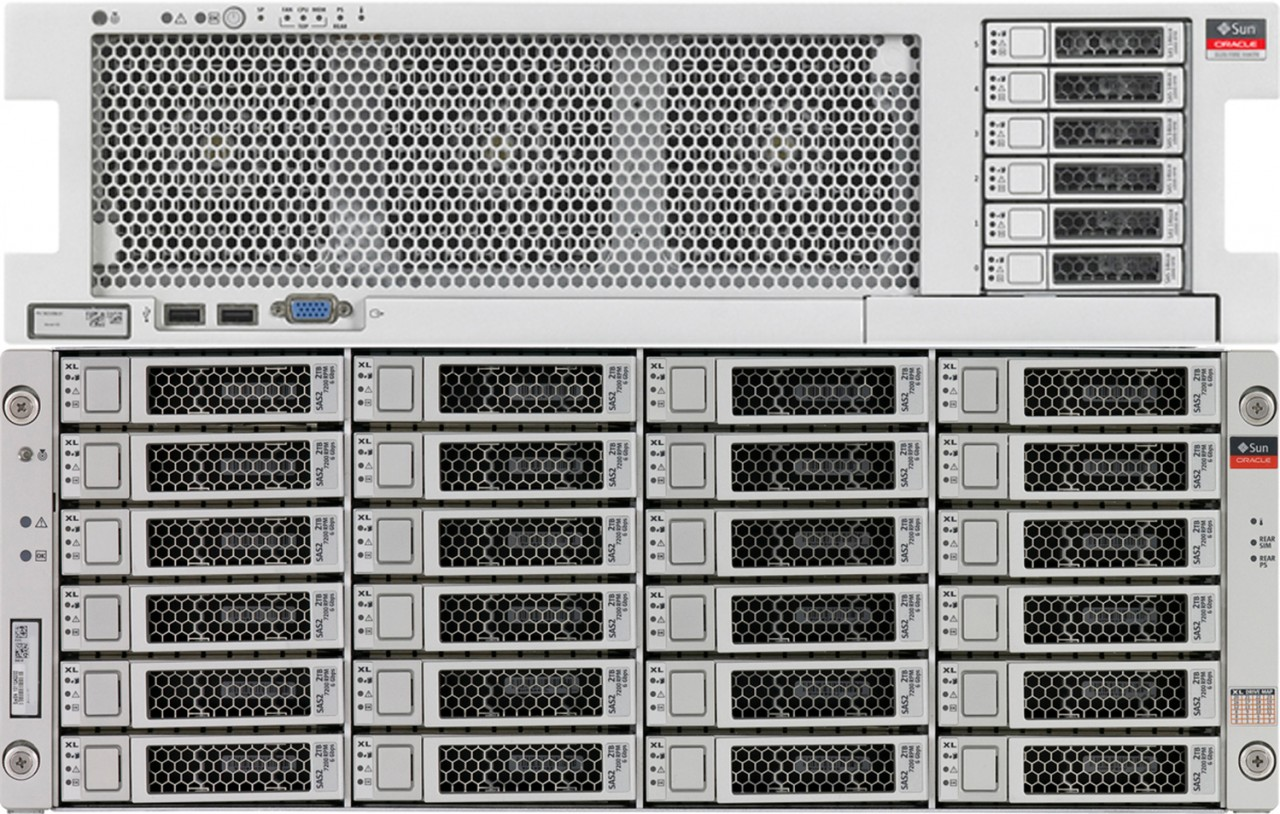
\includegraphics[width=0.7\textwidth]{7420_front_zoom}\\
    \fontsize{3}{3}\selectfont Oracle 
    http://www.e-business.com/zfs-7420-storage-appliance
    \end{center}
\end{frame}

\begin{frame}[fragile]
  \frametitle{future of storage}
    % \begin{itemize}
    %     \item
    % \end{itemize}
    \begin{columns}
        \column{.5\textwidth}
        \tikzset{
  sshadow/.style={opacity=.25, shadow xshift=0.05, shadow yshift=-0.06},
}

%-----TBoxes
%-----#1 height, #2 width, #3 anchor for the label, #4 name of the node, #5
%-----coordinate, #6 label
\def\tboxr[#1,#2,#3,#4,#5]#6{%
  \node[draw, drop shadow={opacity=.35}, minimum height=#1, minimum width=#2, %
  inner color=black!2, outer color=black!2, color=mDarkTeal] (#4) at #5 {}; %
  \node[anchor=#3,inner sep=2pt] at (#4.#3) {#6}; %
}

%-----#1 name of the node, #2 coordinate, #3 label
\def\entity[#1,#2]#3;{
  \node[draw,drop shadow={opacity=.4,shadow xshift=0.04, shadow
    yshift=-0.04},color=mDarkTeal,fill=black!2,rounded corners=3] (#1) at #2 {#3};
}

%-----ABoxes
%-----#1 height, #2 width, #3 aspect, #4 name of the node, #5
%-----coordinate, #6 label
\def\aboxr[#1,#2,#3,#4,#5]#6{%
  \node[draw, cylinder, alias=cyl, shape border rotate=90, aspect=#3, %
  minimum height=#1, minimum width=#2, outer sep=-0.5\pgflinewidth, %
  color=orange!20, left color=mLightBrown, right color=mLightBrown
  ] (#4) at #5 {};%
  \node at #5 {#6};%
  \fill [mLightBrown] let \p1 = ($(cyl.before top)!0.5!(cyl.after top)$), \p2 =
  (cyl.top), \p3 = (cyl.before top), \n1={veclen(\x3-\x1,\y3-\y1)},
  \n2={veclen(\x2-\x1,\y2-\y1)} in (\p1) ellipse (\n1 and \n2); }

\begin{tikzpicture}[
    mnode/.style={circle,draw=black,fill=black,inner sep=0pt,minimum size=0.5pt},
    %scale=0.7
    ]
\small
    \tboxr[40,150,north,stapp,(0,1.5)]{\tiny Support and maintenance};
    \tboxr[40,150,north,stapp,(0,1)]{\tiny Proprietary software};
    \tboxr[40,150,north,stapp,(0,0.5)]{\tiny Proprietary hardware};

    \entity[pc1,(0,0.6)] {\tiny Computer};
    \entity[pc2,(1,0.6)] {\tiny Computer};
    \entity[pc3,(2,0.6)] {\tiny Computer};
    \entity[pc4,(-1,0.6)] {\tiny Computer};
    \entity[pc5,(-2,0.6)] {\tiny Computer};
    \aboxr[10,20,1.2,d1,(0,0)]{\tiny Disk};
    \aboxr[10,20,1.2,d2,(1,0)]{\tiny Disk};
    \aboxr[10,20,1.2,d3,(2,0)]{\tiny Disk};
    \aboxr[10,20,1.2,d4,(-1,0)]{\tiny Disk};
    \aboxr[10,20,1.2,d5,(-2,0)]{\tiny Disk};

    \only<2>{
    \draw[color=red] (-2.64,-0.21) -- (2.64,2.21);
    \draw[color=red] (-2.64, 2.21) -- (2.64,-0.21);
    }

\end{tikzpicture}

        \column{.5\textwidth}
        \only<2>{\tikzset{
  sshadow/.style={opacity=.25, shadow xshift=0.05, shadow yshift=-0.06},
}

%-----TBoxes
%-----#1 height, #2 width, #3 anchor for the label, #4 name of the node, #5
%-----coordinate, #6 label
\def\tboxr[#1,#2,#3,#4,#5]#6{%
  \node[draw, drop shadow={opacity=.35}, minimum height=#1, minimum width=#2, %
  inner color=black!2, outer color=black!2, color=mDarkTeal] (#4) at #5 {}; %
  \node[anchor=#3,inner sep=2pt] at (#4.#3) {#6}; %
}

%-----#1 name of the node, #2 coordinate, #3 label
\def\entity[#1,#2]#3;{
  \node[draw,drop shadow={opacity=.4,shadow xshift=0.04, shadow
    yshift=-0.04},color=mDarkTeal,fill=black!2,rounded corners=3] (#1) at #2 {#3};
}

%-----ABoxes
%-----#1 height, #2 width, #3 aspect, #4 name of the node, #5
%-----coordinate, #6 label
\def\aboxr[#1,#2,#3,#4,#5]#6{%
  \node[draw, cylinder, alias=cyl, shape border rotate=90, aspect=#3, %
  minimum height=#1, minimum width=#2, outer sep=-0.5\pgflinewidth, %
  color=orange!20, left color=mLightBrown, right color=mLightBrown
  ] (#4) at #5 {};%
  \node at #5 {#6};%
  \fill [mLightBrown] let \p1 = ($(cyl.before top)!0.5!(cyl.after top)$), \p2 =
  (cyl.top), \p3 = (cyl.before top), \n1={veclen(\x3-\x1,\y3-\y1)},
  \n2={veclen(\x2-\x1,\y2-\y1)} in (\p1) ellipse (\n1 and \n2); }

\begin{tikzpicture}[
    mnode/.style={circle,draw=black,fill=black,inner sep=0pt,minimum size=0.5pt},
    %scale=0.7
    ]
\small
    \tboxr[10,150,north,stapp,(0,2)]{\tiny Enterprise subscription (optional)\hspace*{0.5cm}
\includegraphics[width=0.1\textwidth]{Inktank}};
    \tboxr[10,150,north,stapp,(0,1.5)]{\tiny Open-source software\hspace*{0.5cm}
\includegraphics[width=0.1\textwidth]{Ceph_logo}};
    \tboxr[40,150,north,stapp,(0,0.5)]{\tiny Commodity hardware};

    \entity[pc1,(0,0.6)] {\tiny Computer};
    \entity[pc2,(1,0.6)] {\tiny Computer};
    \entity[pc3,(2,0.6)] {\tiny Computer};
    \entity[pc4,(-1,0.6)] {\tiny Computer};
    \entity[pc5,(-2,0.6)] {\tiny Computer};
    \aboxr[10,20,1.2,d1,(0,0)]{\tiny Disk};
    \aboxr[10,20,1.2,d2,(1,0)]{\tiny Disk};
    \aboxr[10,20,1.2,d3,(2,0)]{\tiny Disk};
    \aboxr[10,20,1.2,d4,(-1,0)]{\tiny Disk};
    \aboxr[10,20,1.2,d5,(-2,0)]{\tiny Disk};
    
\end{tikzpicture}
}
    \end{columns}
\end{frame}


\section{ceph}
\begin{frame}[fragile]
  \frametitle{ceph}
    \begin{columns}
        \column{.5\textwidth}
            \begin{block}{Philosophy}
                \begin{itemize}[<+->]
                \item open-source
                \item community focused
                \item software-defined
                \item scale-out hardware
                \item self-managing
                \item failure is normal
                \end{itemize}
            \end{block}
        \column{.5\textwidth}
            \only<7->{
            \begin{block}{History}
                \begin{center}
                \tikzset{
  sshadow/.style={opacity=.25, shadow xshift=0.05, shadow yshift=-0.06},
}
%-----#1 name of the node, #2 coordinate, #3 label
\def\entity[#1,#2]#3;{
  \node[draw,drop shadow={opacity=.4,shadow xshift=0.04, shadow
    yshift=-0.04},color=mDarkTeal,fill=black!2,rounded corners=3] (#1) at #2 {#3};
}

\begin{tikzpicture}[
    mnode/.style={circle,draw=black,fill=black,inner sep=0pt,minimum size=0.5pt},
    %scale=0.7
    ]
\small
    \draw[color=mLightBrown, fill=mLightBrown] (-1,-0.3) -- (3.8,2.3) -- (4.5,2.3) -- (2.3,-0.3) -- (-1,-0.3);
    \node[color=orange!20] at (1.2,0) {\tiny 2004};
    \node[color=orange!20] at (2.1,0.5) {\tiny 2006};
    \node[color=orange!20] at (2.75,1) {\tiny 2010};
    \node[color=orange!20] at (3.5,1.5) {\tiny 2012};
    \node[color=orange!20] at (3.9,2) {\tiny 2014};

    \only<8->{\entity[h1,(0,0)] {\tiny PhD thesis at UCSC};}
    \only<9->{\entity[h2,(0.7,0.5)] {\tiny Project is open-sourced};}
    \only<10->{\entity[h3,(1.4,1)] {\tiny Included in Linux kernel};}
    \only<11->{\entity[h4,(2.1,1.5)] {\tiny Integrated into CloudStack};}
    \only<12->{\entity[h5,(2.8,2)] {\tiny RedHat acquisition};}
    
\end{tikzpicture}

            \end{center}
            \end{block}
            }
    \end{columns}
\end{frame}

\begin{frame}[fragile]
    \frametitle{ceph architecture}
    \begin{center}
        \alt<2>{
        \tikzset{
  sshadow/.style={opacity=.25, shadow xshift=0.05, shadow yshift=-0.06},
}

%-----TBoxes
%-----#1 height, #2 width, #3 anchor for the label, #4 name of the node, #5
%-----coordinate, #6 label
\def\tboxr[#1,#2,#3,#4,#5]#6{%
  \node[draw, drop shadow={opacity=.35}, minimum height=#1, minimum width=#2, %
  inner color=black!2, outer color=black!2, color=mDarkTeal] (#4) at #5 {}; %
  \node[anchor=#3,inner sep=2pt, align=center] at (#4.#3) {#6}; %
}

%-----#1 name of the node, #2 coordinate, #3 label
\def\entity[#1,#2]#3;{
  \node[draw,drop shadow={opacity=.4,shadow xshift=0.04, shadow
    yshift=-0.04},color=mDarkTeal,fill=black!2,rounded corners=3] (#1) at #2 {#3};
}

%-----#1 from node, #2 to node, #3 specification of a node (label), #4
%-----dashed, or other parameters for draw
\def\isaedge[#1,#2,#3,#4];{ 
  \draw[to-to,color=mDarkTeal,#4,fill=mDarkTeal] (#1) -- #3
  (#2);  
}

\begin{tikzpicture}[
    mnode/.style={circle,draw=black,fill=black,inner sep=0pt,minimum size=0.5pt},
    %scale=0.7
    ]
\small
    \node [mnode] (pt1) at (-0.75, 1.625) {};
    \tboxr[60,70,north,gw,(1.22,2.25)]{
        \tiny \textbf{RADOSGW}\\
        \tiny bucket-based REST gateway\\
        \tiny S3- and Swift-compatible
    };
    \tboxr[60,60,north,rbd,(3.4,2.25)]{
        \tiny \textbf{RBD}\\
        \tiny virtual block device\\
        \tiny Linux kernel client\\
        \tiny QEMU/KVM driver
    };
    \node[draw,drop shadow={opacity=.4,shadow xshift=0.04, shadow
        yshift=-0.04},color=mDarkTeal,fill=mLightBrown!20,rounded corners=3,
        minimum height=35, minimum width=175, align=center] 
        (librados) at (1.5,1) {
            \tiny \textbf{librados}\\
            \tiny allows apps direct access to RADOS\\
            \tiny support for C, C++, Java, Python, Ruby, PHP
        };
    \tboxr[88.5,60,north,fs,(5.5,1.75)]{
        \tiny \textbf{CephFS}\\
        \tiny POSIX-compliant\\
        \tiny Linux kernel client\\
        \tiny FUSE support
    };

    \node[draw,drop shadow={opacity=.4,shadow xshift=0.04, shadow
        yshift=-0.04},color=mLightBrown!20,fill=mLightBrown,rounded corners=3,
        minimum height=20, minimum width=240, align=center] 
        (rados) at (2.5,-0.25) {
            \tiny \textbf{RADOS}\\
            \tiny A reliable, autonomous, distributed object store\\
            \tiny consisting of self-healing, self-managing, intelligent storage nodes
        };

    \entity[cl1,(-0.75,4)]{\tiny Application};
    \entity[cl2,(1.22,4)]{\tiny REST};
    \entity[cl3,(3.4,4)]{\tiny Host/VM};
    \entity[cl4,(5.5,4)]{\tiny FS client};

    \isaedge[cl1, pt1,,];
    \isaedge[cl2, gw,,];
    \isaedge[cl3, rbd,,];
    \isaedge[cl4, fs,,];

\end{tikzpicture}

        }{
        \tikzset{
  sshadow/.style={opacity=.25, shadow xshift=0.05, shadow yshift=-0.06},
}

%-----TBoxes
%-----#1 height, #2 width, #3 anchor for the label, #4 name of the node, #5
%-----coordinate, #6 label
\def\tboxr[#1,#2,#3,#4,#5]#6{%
  \node[draw, drop shadow={opacity=.35}, minimum height=#1, minimum width=#2, %
  inner color=black!2, outer color=black!2, color=mDarkTeal] (#4) at #5 {}; %
  \node[anchor=#3,inner sep=2pt, align=center] at (#4.#3) {#6}; %
}

%-----#1 name of the node, #2 coordinate, #3 label
\def\entity[#1,#2]#3;{
  \node[draw,drop shadow={opacity=.4,shadow xshift=0.04, shadow
    yshift=-0.04},color=mDarkTeal,fill=black!2,rounded corners=3] (#1) at #2 {#3};
}

\begin{tikzpicture}
\small
    \draw[dashed,to-to,color=mDarkTeal,fill=mDarkTeal] (0,1.5) -- (0,4);
    \draw[dashed,to-to,color=mDarkTeal,fill=mDarkTeal] (2.5,1.5) -- (2.5,4);
    \draw[dashed,to-to,color=mDarkTeal,fill=mDarkTeal] (5,1.5) -- (5,4);
    
    \tboxr[40,60,north,gw,(0,1)]{
        \tiny \textbf{Ceph Object Gateway}\\
        \tiny S3- and Swift-compatible
    };
    \tboxr[40,60,north,rbd,(2.5,1)]{
        \tiny \textbf{Ceph Block Device}\\
        \tiny virtual block device
    };
    \tboxr[40,60,north,fs,(5,1)]{
        \tiny \textbf{Ceph Filesystem}\\
        \tiny POSIX-compliant\\
    };

    \node[draw,drop shadow={opacity=.4,shadow xshift=0.04, shadow
        yshift=-0.04},color=mLightBrown!20,fill=mLightBrown,rounded corners=3,
        minimum height=20, minimum width=240, align=center] 
        (rados) at (2.5,0) {
            \tiny \textbf{Ceph storage cluster}\\
            \tiny A reliable, easy to manage, distributed object store
        };

    \entity[cl1,(0,3)]{\tiny Objects};
    \entity[cl2,(2.5,3)]{\tiny Virtual disks};
    \entity[cl3,(5,3)]{\tiny Files and directories};

\end{tikzpicture}

        }
    \end{center}
\end{frame}

\begin{frame}[fragile]
    \frametitle{rados}
    \begin{center}
        \tikzset{
  sshadow/.style={opacity=.25, shadow xshift=0.05, shadow yshift=-0.06},
}

%-----TBoxes
%-----#1 height, #2 width, #3 anchor for the label, #4 name of the node, #5
%-----coordinate, #6 label
\def\osd[#1,#2,#3,#4,#5]{%
  \node[draw, drop shadow={opacity=.35}, minimum height=#1, minimum width=#2, %
  inner color=black!2, outer color=black!2, color=mDarkTeal] (#4) at #5 {}; %
  \node[anchor=#3,inner sep=2pt,color=mDarkTeal] at (#4.#3) {\tiny OSD}; %
}
%-----#1 height, #2 width, #3 anchor for the label, #4 name of the node, #5
%-----coordinate, #6 label
\def\mon[#1,#2,#3,#4,#5]{%
  \node[draw, drop shadow={opacity=.35}, minimum height=#1, minimum width=#2, %
  inner color=mLightBrown!20, outer color=mLightBrown!20, color=mDarkTeal] (#4) at #5 {}; %
  \node[anchor=#3,inner sep=2pt,color=mDarkTeal] at (#4.#3) {\tiny MON}; %
}
%-----ABoxes
%-----#1 height, #2 width, #3 aspect, #4 name of the node, #5
%-----coordinate, #6 label
\def\disk[#1,#2,#3,#4,#5]#6{%
  \node[draw, cylinder, alias=cyl, shape border rotate=90, aspect=#3, %
  minimum height=#1, minimum width=#2, outer sep=-0.5\pgflinewidth, %
  color=orange!20, left color=mLightBrown, right color=mLightBrown
  ] (#4) at #5 {};%
  \node at #5 {#6};%
  \fill [mLightBrown] let \p1 = ($(cyl.before top)!0.5!(cyl.after top)$), \p2 =
  (cyl.top), \p3 = (cyl.before top), \n1={veclen(\x3-\x1,\y3-\y1)},
  \n2={veclen(\x2-\x1,\y2-\y1)} in (\p1) ellipse (\n1 and \n2); }

%-----#1 height, #2 width, #3 name of the node, #4
%-----coordinate, #5 label
\def\kbbox[#1,#2,#3,#4,#5]#6{
        \draw[dashed] node[draw,color=gray!50,minimum
        height=#1,minimum width=#2] (#4) at #5 {}; 
        \node[anchor=#3,inner sep=2pt] at (#4.#3)  {#6};
}

\begin{tikzpicture}
\small

    \osd[20,20,north,osd6,(-4,0.2)];
    \osd[20,20,north,osd6,(-4,1.2)];
    \osd[20,20,north,osd6,(-3,0.2)];
    \mon[20,20,center,mon2,(-3,1.2)];
    \osd[20,20,north,osd4,(-2,0.2)];
    \osd[20,20,north,osd6,(-2,1.2)];
    \osd[20,20,north,osd3,(-1,0.2)];
    \osd[20,20,north,osd6,(-1,1.2)];
    \osd[20,20,north,osd1,(0,0.2)];
    \osd[20,20,north,osd6,(0,1.2)];
    \mon[20,20,center,mon1,(1,0.2)];
    \osd[20,20,north,osd6,(1,1.2)];
    \osd[20,20,north,osd2,(2,0.2)];
    \osd[20,20,north,osd6,(2,1.2)];
    \osd[20,20,north,osd5,(3,0.2)];
    \osd[20,20,north,osd6,(3,1.2)];
    \osd[20,20,north,osd6,(4,0.2)];
    \mon[20,20,center,mon3,(4,1.2)];

    \disk[10,15,1,d6,(-4,0)]{};
    \disk[10,15,1,d6,(-4,1)]{};
    \disk[10,15,1,d6,(-3,0)]{};
    \disk[10,15,1,d4,(-2,0)]{};
    \disk[10,15,1,d4,(-2,1)]{};
    \disk[10,15,1,d3,(-1,0)]{};
    \disk[10,15,1,d3,(-1,1)]{};
    \disk[10,15,1,d1,(0,0)]{};
    \disk[10,15,1,d1,(0,1)]{};
    \disk[10,15,1,d6,(1,1)]{};
    \disk[10,15,1,d2,(2,0)]{};
    \disk[10,15,1,d2,(2,1)]{};
    \disk[10,15,1,d5,(3,0)]{};
    \disk[10,15,1,d5,(3,1)]{};
    \disk[10,15,1,d6,(4,0)]{};

    \kbbox[60,260,1,rados,(0,0.7)]{};
    
\end{tikzpicture}

    \end{center}
\end{frame}

\begin{frame}[fragile]
    \frametitle{ceph daemons}
    \begin{columns}
        \column{.5\textwidth}
            \begin{block}{OSD}
                \begin{itemize}
                \item serve objects to clients
                \item one per disk
                \item backend: btrfs, xfs, ext4
                \item peer-to-peer replication and recovery
                \item write-ahead journal
            \end{itemize}
            \end{block}
        \column{.5\textwidth}
            \begin{block}{MON}
                \begin{itemize}
                \item maintain cluster state and membership
                \item vote for distributed decision-making
                \item small, odd number
                \end{itemize}
                \vspace*{8mm}
            \end{block}
    \end{columns}
\end{frame}

\section{data placement}
\begin{frame}[fragile]
    \frametitle{hotels}
    \begin{center}
        \only<1>{
        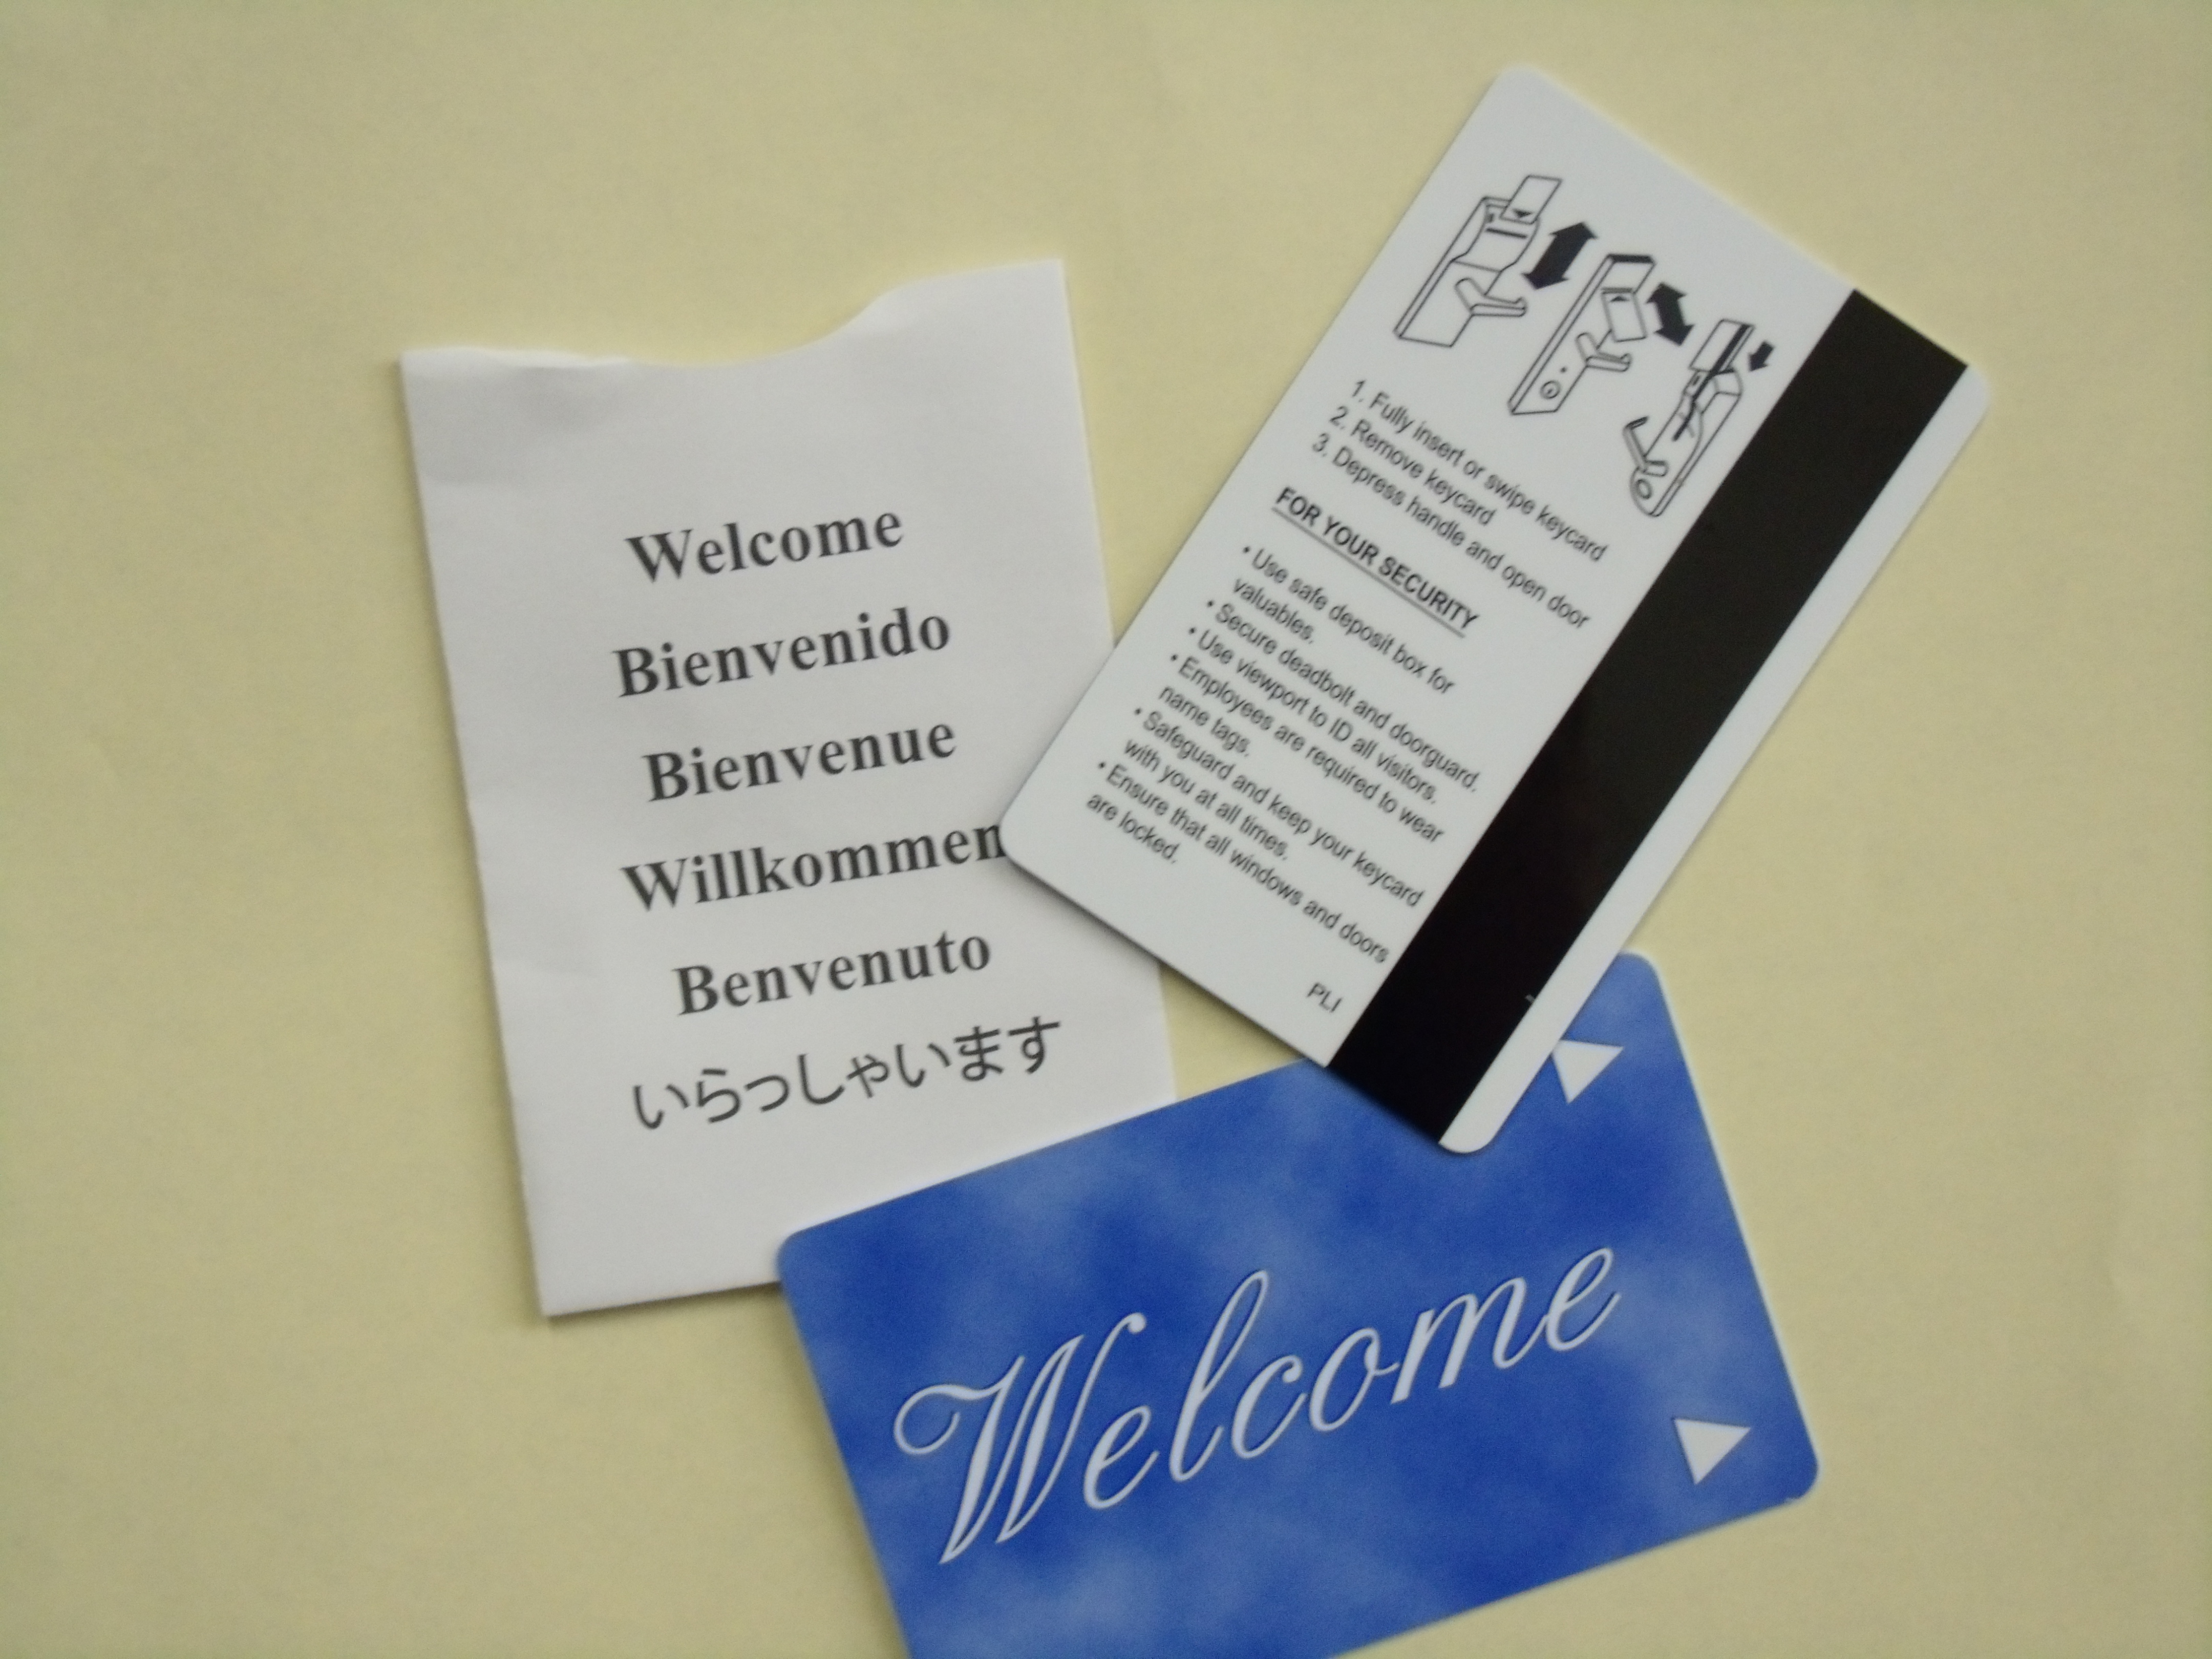
\includegraphics[width=.6\textwidth]{Generic-Key-Card}\\
        \fontsize{3}{3}\selectfont 
    http://free-stock-illustration.com/hotel+key+card
        }
        \only<2>{
        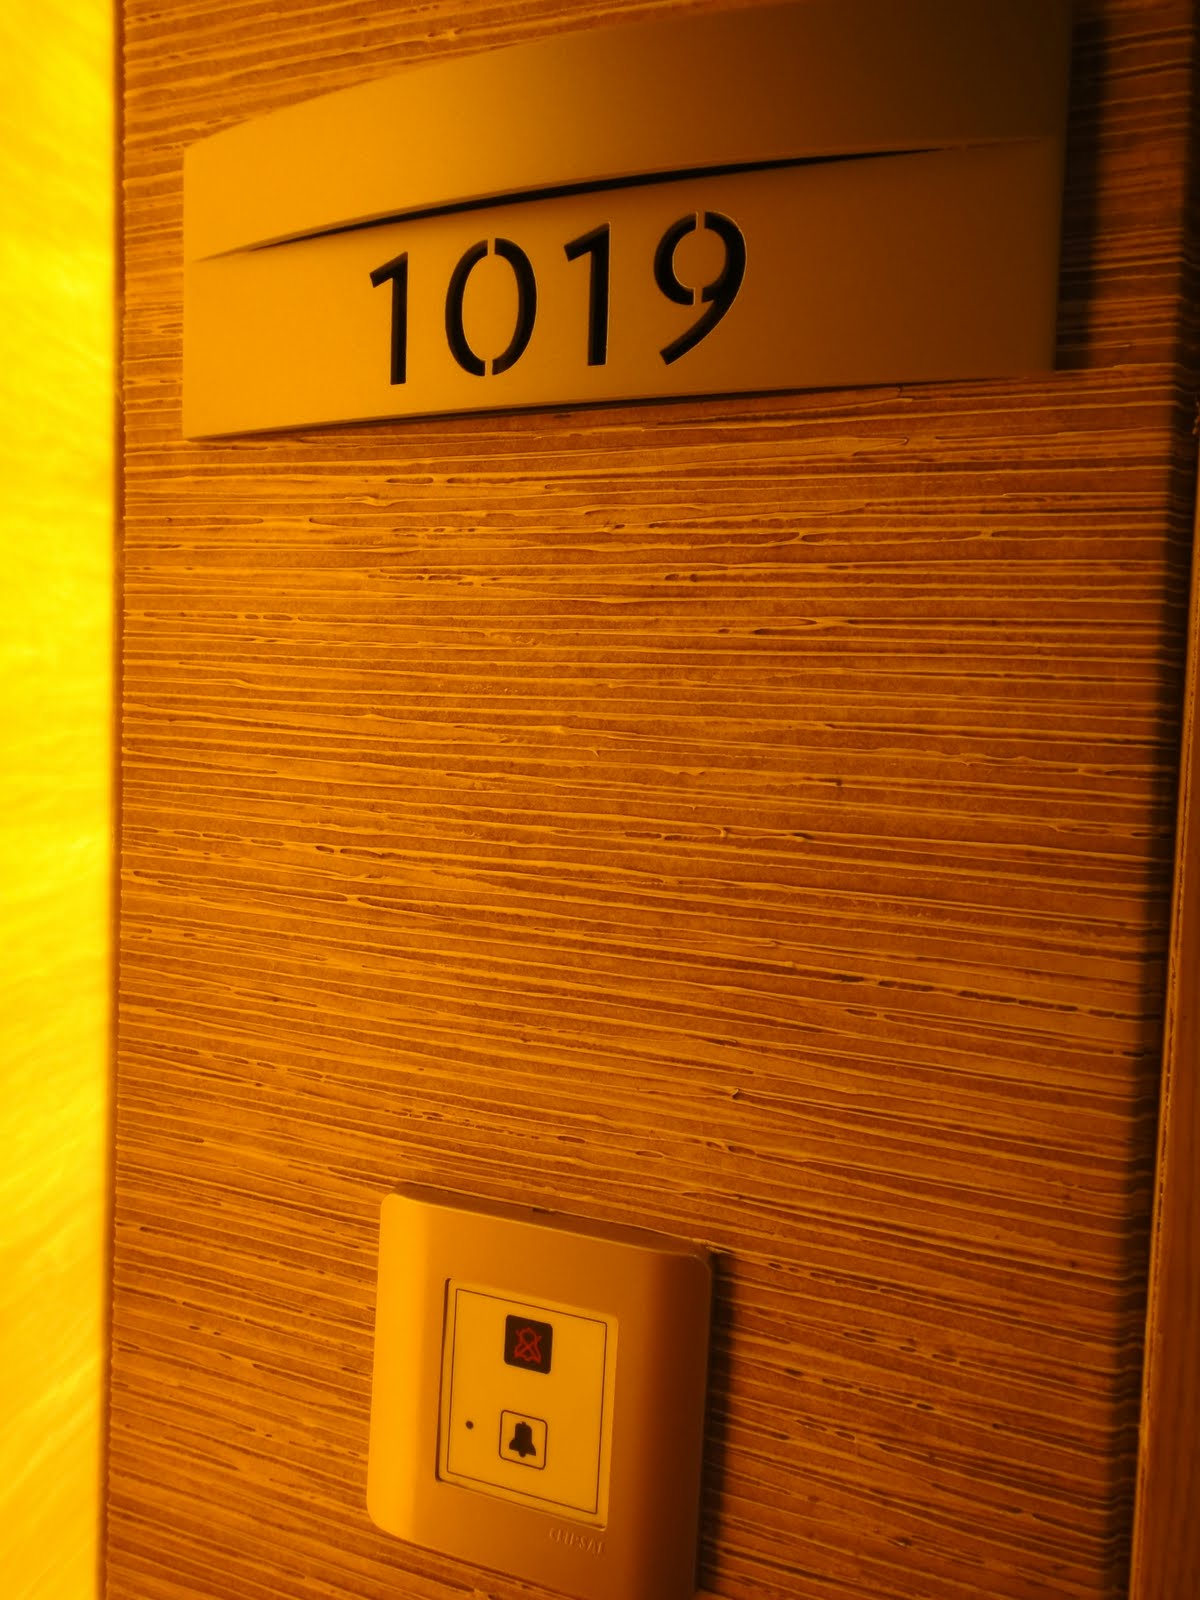
\includegraphics[width=.5\textwidth]{hotel-room-2}\\
        \fontsize{3}{3}\selectfont 
    % http://www.letterlux.com/wp-content/uploads/2014/09/illuminated-hotel-room-numbers.jpg
    http://2.bp.blogspot.com/-o-rlIrv094E/TXxj8D-B2LI/AAAAAAAAGh8/VEbrbHpxVxo/s1600/DSC02213.JPG
        }
        \only<3>{
            \begin{itemize}
                \item What if the hotel had 1 billion rooms? Or $\infty$?
            \end{itemize}
            \alert{\#13,565,983}
        }
        \only<4>{
            %\begin{itemize}
            %    \item
            What if the hotel changed constantly?
            %\end{itemize}
        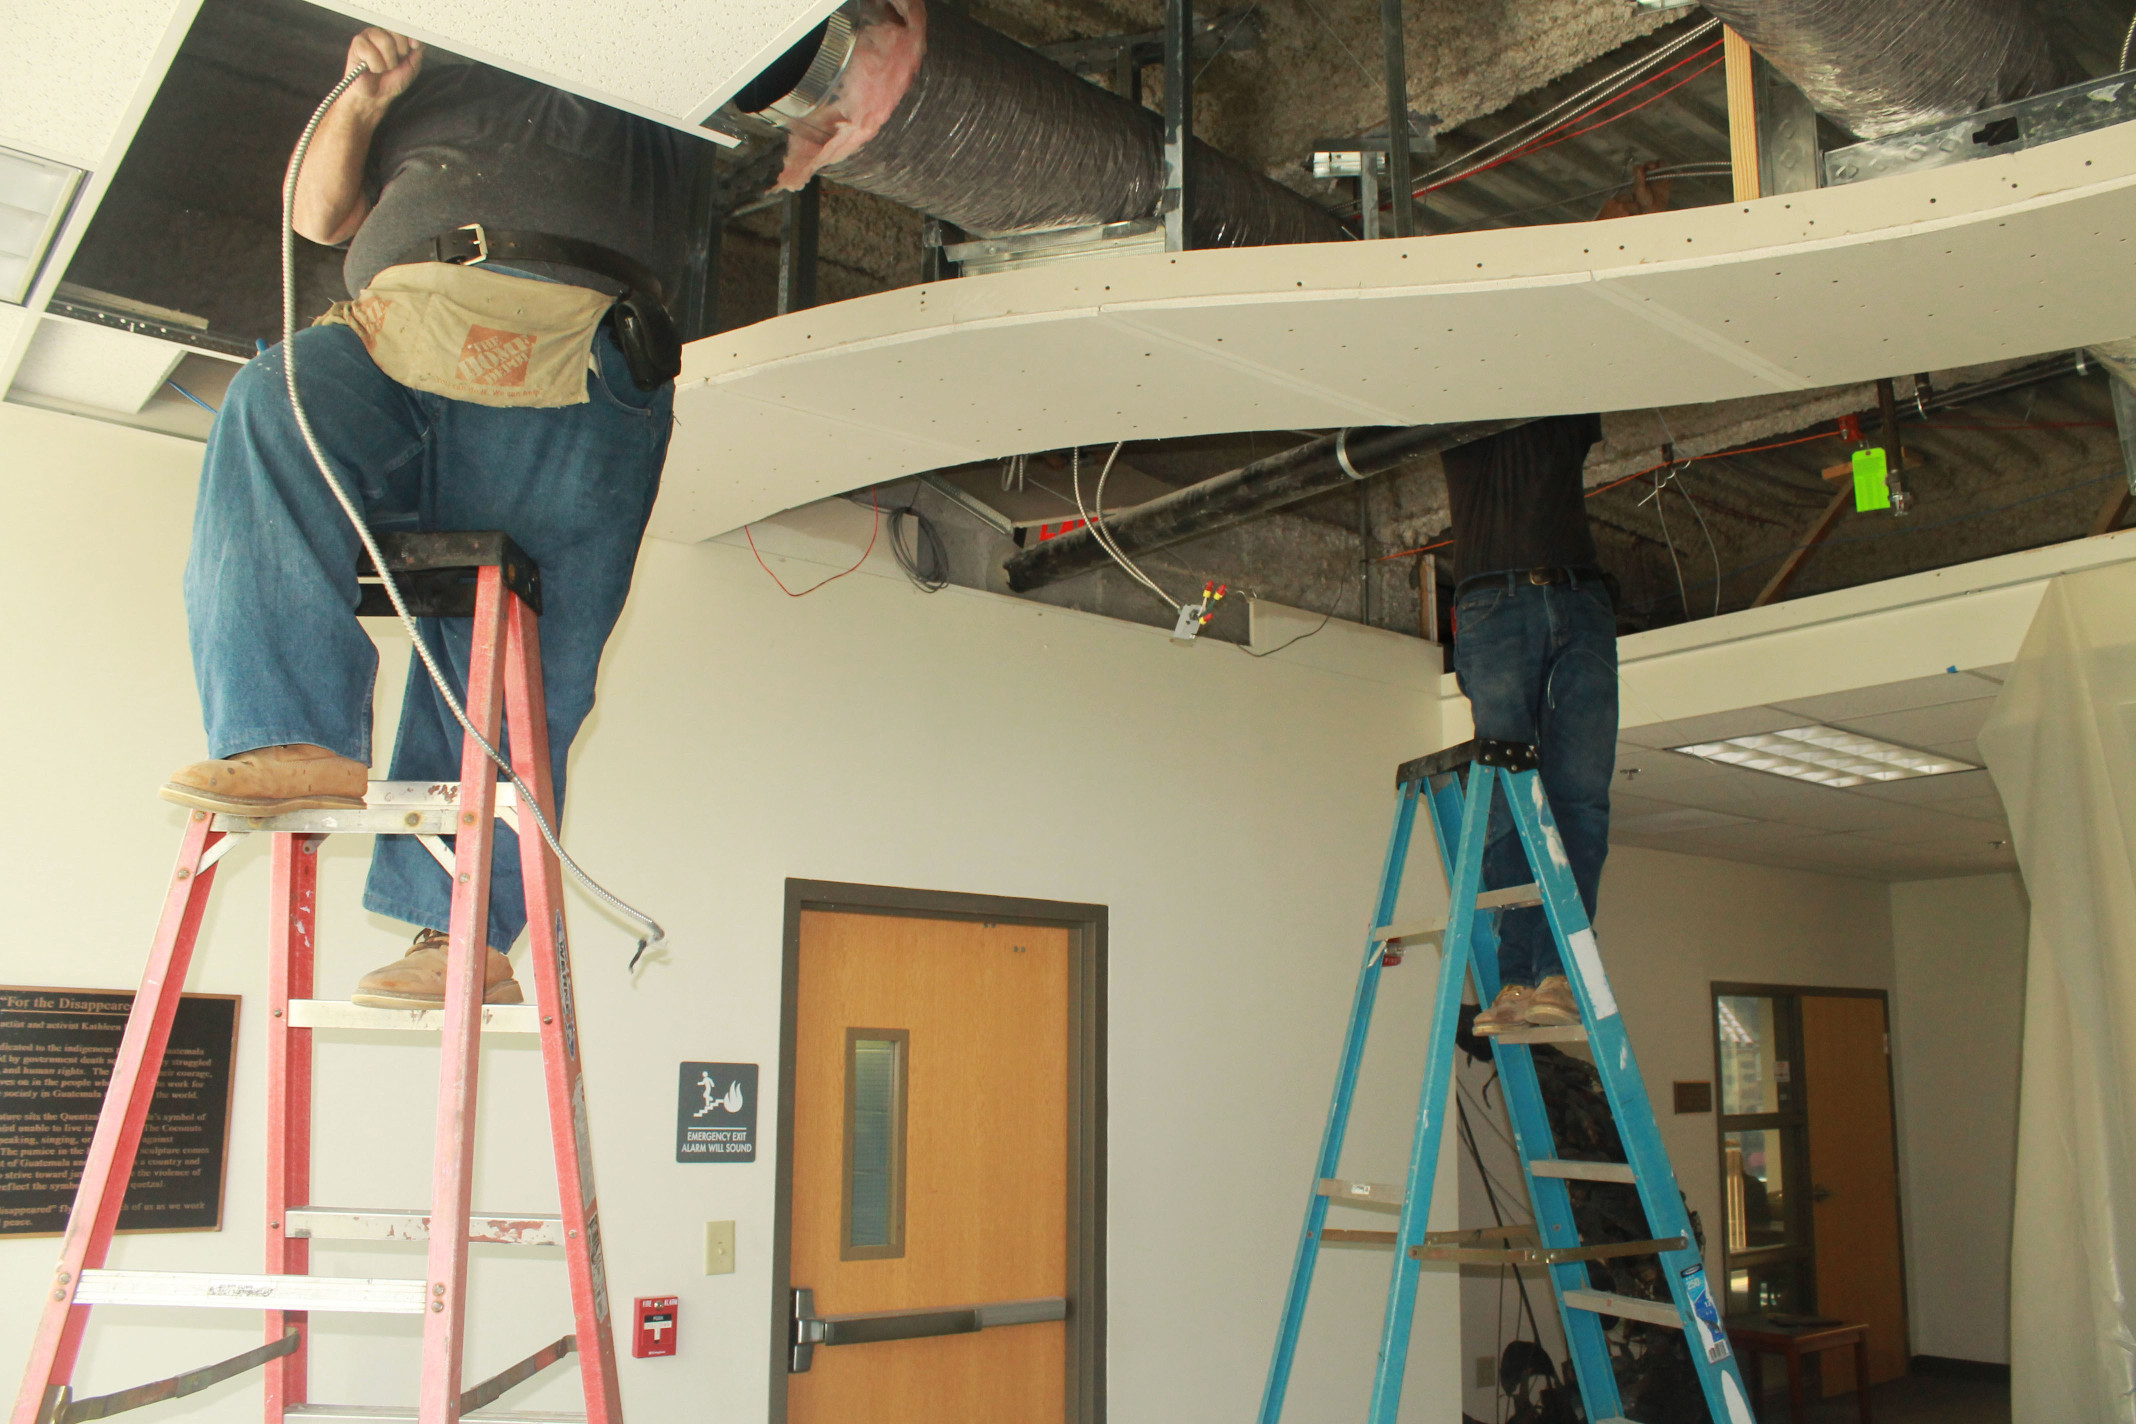
\includegraphics[width=.75\textwidth]{renovation-1}\\
        \fontsize{3}{3}\selectfont 
            http://waltonian.com/news/eastern-library-renovations-continue/
        }
        \only<5>{
            %\begin{itemize}
                %\item
            Scale-up everything?
            %\end{itemize}
        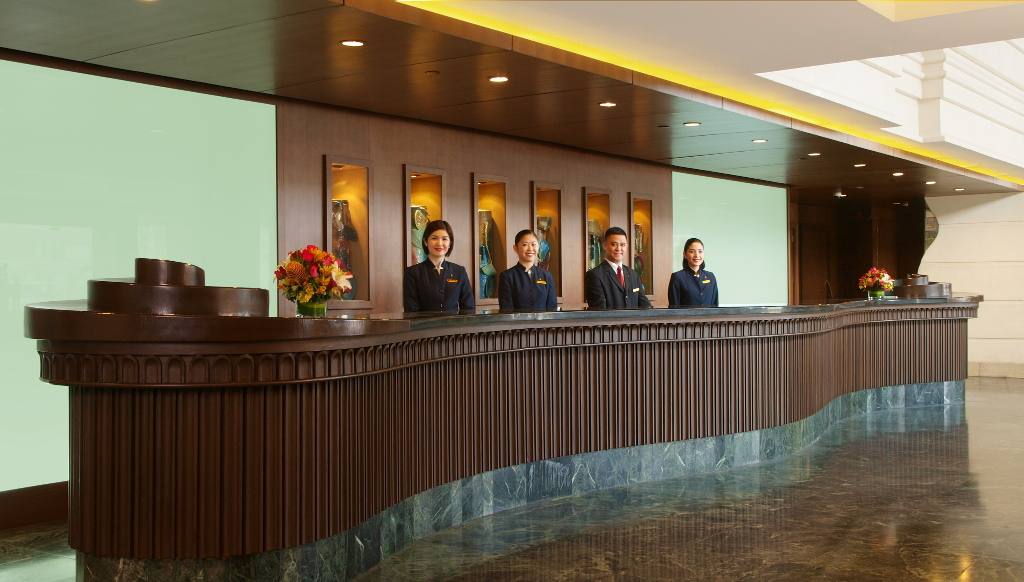
\includegraphics[width=.75\textwidth]{hotel-reception}\\
        \fontsize{3}{3}\selectfont 
    http://www.millenniumhotels.com/content/dam/global/en/the-heritage-hotel-manila/images/cons-photographics-lobby-reception-desk\%2003062011\_34-basicB-preview-2048.jpg
        }
    \end{center}
    \only<6->{
        \begin{itemize}
            \item<6-> The hotel itself must assign people to rooms instead of a
                centralized place
            \item<6-> The hotel should grow itself organically
            \item<7-> \alert{Deterministic placement algorithm}
            \item<7-> \alert{Intelligent nodes}
        \end{itemize}
    }
\end{frame}

\begin{frame}[fragile]
    \frametitle{crush}
    \begin{center}
        \tikzset{
  sshadow/.style={opacity=.25, shadow xshift=0.05, shadow yshift=-0.06},
}

%-----#1 size, #2 angle, #3 aspect, #4 label next to the diamond
%-----#5 name of the node, #6 coordinate, #7 label
\def\schemer[#1,#2,#3,#4,#5,#6]#7{ %
  \node[draw, diamond, shape aspect=#3, rotate=#2, minimum size=#1, %
  bottom color=green!65, top color=green!30, color=green!60!black, %
  drop shadow={sshadow,color=green!65!black}, #4] (#5) at #6
  {\textcolor{green!53}{bla}}; %
  \node at #6 {#7}; %
}

%-----TBoxes
%-----#1 height, #2 width, #3 anchor for the label, #4 name of the node, #5
%-----coordinate, #6 label
\def\tboxr[#1,#2,#3,#4,#5]#6{%
  \node[draw, drop shadow={opacity=.35}, minimum height=#1, minimum width=#2, %
  inner color=black!2, outer color=black!2, color=mDarkTeal] (#4) at #5 {}; %
  \node[anchor=#3,inner sep=2pt,align=center] at (#4.#3) {#6}; %
}
\def\osd[#1,#2,#3,#4,#5]#6{%
  \node[draw, drop shadow={opacity=.35}, minimum height=#1, minimum width=#2, %
  inner color=black!2, outer color=black!2, color=mDarkTeal] (#4) at #5 {}; %
  \node[anchor=#3,inner sep=2pt] at (#4.#3) {#6}; %
}

%-----#1 name of the node, #2 coordinate, #3 label
\def\entity[#1,#2]#3;{
  \node[draw,align=center,drop shadow={opacity=.4,shadow xshift=0.04, shadow
    yshift=-0.04},color=mDarkTeal,fill=mLightBrown!20,rounded corners=3] (#1) at #2 {#3};
}
\def\ragent[#1,#2]#3;{
  \node[draw,drop shadow={opacity=.4,shadow xshift=0.04, shadow
    yshift=-0.04},color=mDarkTeal,fill=mLightBrown!20,rounded corners=3] (#1) at #2 {#3};
}
\def\cagent[#1,#2]#3;{
  \node[draw,drop shadow={opacity=.4,shadow xshift=0.04, shadow
    yshift=-0.04},color=mDarkTeal,fill=mDarkTeal!20,rounded corners=3] (#1) at #2 {#3};
}

%-----#1 from node, #2 to node, #3 specification of a node (label), #4
%-----dashed, or other parameters for draw
\def\isaedge[#1,#2,#3,#4];{ 
  \draw[to-to,color=mDarkTeal,#4,fill=mDarkTeal] (#1) -- #3
  (#2);  
}

%-----ABoxes
%-----#1 height, #2 width, #3 aspect, #4 name of the node, #5
%-----coordinate, #6 label
\def\disk[#1,#2,#3,#4,#5]#6{%
  \node[draw, cylinder, alias=cyl, shape border rotate=90, aspect=#3, %
  minimum height=#1, minimum width=#2, outer sep=-0.5\pgflinewidth, %
  color=orange!20, left color=mLightBrown, right color=mLightBrown
  ] (#4) at #5 {};%
  \node at #5 {#6};%
  \fill [mLightBrown] let \p1 = ($(cyl.before top)!0.5!(cyl.after top)$), \p2 =
  (cyl.top), \p3 = (cyl.before top), \n1={veclen(\x3-\x1,\y3-\y1)},
  \n2={veclen(\x2-\x1,\y2-\y1)} in (\p1) ellipse (\n1 and \n2); }

%-----#1 height, #2 width, #3 name of the node, #4
%-----coordinate, #5 label
\def\kbbox[#1,#2,#3,#4,#5]#6{
        \draw[dashed] node[draw,color=gray!50,minimum
        height=#1,minimum width=#2] (#4) at #5 {}; 
        \node[anchor=#3,inner sep=2pt] at (#4.#3)  {#6};
}

%-----#1 from node, #2 to node, #3 specification of a node (label), #4
%-----dashed, or other parameters for draw
\def\soledge[#1,#2,#3,#4];{
        \draw[dashed,to-to,color=mDarkTeal,fill=mDarkTeal,#4] (#1) -- #3 (#2);
}

\begin{tikzpicture}[
    mnode/.style={circle,draw=black,fill=black,inner sep=0pt,minimum size=0.5pt},
    %scale=0.7
    ]
\small
%    \tboxr[10,150,north,stapp,(0,2)]{\tiny Enterprise subscription (optional)\hspace*{0.5cm}
\includegraphics[width=0.1\textwidth]{Inktank}};
%    \entity[pc1,(0,0.6)] {\tiny Computer};

    \tboxr[8,60,north,obj,(0,4.5)] {\tiny 011101010100011010101010};
    \tboxr[8,40,north,pg,(0,3)] {\tiny placement group};
    
    \osd[20,20,north,osd1,(0,1.2)]{\tiny OSD};
    \osd[16,16,north,osd2,(-0.5,0.15)]{\tiny OSD};
    \osd[16,16,north,osd3,(0.5,0.15)]{\tiny OSD};
    \disk[10,15,1,d1,(0,1)]{};
    \disk[5,12,0.5,d2,(-0.5,0)]{};
    \disk[5,12,0.5,d3,(0.5,0)]{};
    \draw[->,color=mDarkTeal] (osd1) -- (-0.5,1.2) -- (osd2);
    \draw[->,color=mDarkTeal] (osd1) -- (0.5,1.2) -- (osd3);

    \draw[->,dashed,color=mDarkTeal] (obj) -- (pg);
    \draw[->,dashed,color=mDarkTeal] (pg) -- (osd1);

    \entity[hash,(0.95,3.75)]{\tiny hash obj id + pool};
    \entity[crush,(0.5,2.25)]{\tiny CRUSH};

    \only<2>{
    \tboxr[20,30,north,egobj,(4,4.7)]{\tiny obj='foo'\\\tiny pool='bar'};
    \tboxr[8,40,north,egpg,(4,3)]{\tiny 5.23};
    \draw[->,dashed,color=mDarkTeal] (egobj) -- (egpg);
    \entity[eghash1,(5.13,3.9)]{\tiny hash('foo') \% 256 = 0x23};
    \entity[eghash2,(4.5,3.5)]{\tiny 'bar' = 5};
    \entity[egcrush,(5.05,2.25)]{\tiny crush(5.23) = [2, 14, 29]};
    \osd[20,20,north,egosd1,(4,1.2)]{\tiny osd.2};
    \osd[16,16,north,egosd2,(3.5,0.15)]{\tiny osd.14};
    \osd[16,16,north,egosd3,(4.5,0.15)]{\tiny osd.29};
    \disk[10,15,1,egd1,(4,1)]{};
    \disk[5,12,0.5,egd2,(3.5,0)]{};
    \disk[5,12,0.5,egd3,(4.5,0)]{};
    \draw[->,color=mDarkTeal] (egosd1) -- (3.5,1.2) -- (egosd2);
    \draw[->,color=mDarkTeal] (egosd1) -- (4.5,1.2) -- (egosd3);
    \draw[->,dashed,color=mDarkTeal] (egpg) -- (egosd1);
    }

\end{tikzpicture}

    \end{center}
\end{frame}

\begin{frame}[fragile]
    \frametitle{crush}
    \begin{block}{\alert{C}ontrolled \alert{R}eplication \alert{U}nder 
        \alert{S}calable \alert{H}ashing}
    \begin{itemize}
        \item Pseudo-random placement algorithm
        \item Repeatable, deterministic
        \item Statistically uniform distribution
        \item Stable mapping: minimal data migration
        \item Rule-based configuration, topology aware
    \end{itemize}
    \only<1>{\vspace*{35mm}}
    \only<2>{
    \begin{center}
        \begin{tikzpicture}
    \node[draw,color=mDarkTeal] (rack) at (3,2) {\tiny rack bucket};

    \node[draw,color=mDarkTeal] (host1) at (1,1) {\tiny host bucket};
    \node[draw,color=mDarkTeal] (host2) at (5,1) {\tiny host bucket};

    \node[draw,color=mDarkTeal] (osd1) at (0,0) {\tiny osd bucket};
    \node[draw,color=mDarkTeal] (osd2) at (2,0) {\tiny osd bucket};
    \node[draw,color=mDarkTeal] (osd3) at (4,0) {\tiny osd bucket};
    \node[draw,color=mDarkTeal] (osd4) at (6,0) {\tiny osd bucket};

    \draw[color=mDarkTeal] (rack) -- (3,1.5) -- (1,1.5) -- (host1);
    \draw[color=mDarkTeal] (rack) -- (3,1.5) -- (5,1.5) -- (host2);

    \draw[color=mDarkTeal] (host1) -- (1,0.5) -- (0,0.5) -- (osd1);
    \draw[color=mDarkTeal] (host1) -- (1,0.5) -- (2,0.5) -- (osd2);
    \draw[color=mDarkTeal] (host2) -- (5,0.5) -- (4,0.5) -- (osd3);
    \draw[color=mDarkTeal] (host2) -- (5,0.5) -- (6,0.5) -- (osd4);
\end{tikzpicture}

    \end{center}
    }
\end{block}
\end{frame}

\section{ceph clients}
\begin{frame}[fragile]
    \frametitle{librados}
    \begin{itemize}
        \item direct access to RADOS for applications
        \item C, C++, Python, Java, Erlang, PHP
        \item native socket access, no HTTP overhead
    \end{itemize}
\end{frame}

\begin{frame}[fragile]
    \frametitle{radosgw}
    \begin{itemize}
        \item RESTful API
        \item unified object namespace
        \item S3 and Swift compatible
        \item user database and access control
        \item usage accounting, billing
    \end{itemize}
\end{frame}

\begin{frame}[fragile]
    \frametitle{rbd}
    \begin{itemize}
        \item Storage of disk images in RADOS
        \item Images are striped across the cluster
        \item Decoupling of VMs from host
        \item Thin provisioning
            \begin{itemize}
                \item physical storage only used once you begin writing
            \end{itemize}
        \item Snaphots, copy-on-write clones
        \item Support in Qemu, KVM
    \end{itemize}
\end{frame}

\begin{frame}[fragile]
    \frametitle{CephFS}
    \begin{center}
        \tikzset{
  sshadow/.style={opacity=.25, shadow xshift=0.05, shadow yshift=-0.06},
}

%-----TBoxes
%-----#1 height, #2 width, #3 anchor for the label, #4 name of the node, #5
%-----coordinate, #6 label
\def\osd[#1,#2,#3,#4,#5]{%
  \node[draw, drop shadow={opacity=.35}, minimum height=#1, minimum width=#2, %
  inner color=black!2, outer color=black!2, color=mDarkTeal] (#4) at #5 {}; %
  \node[anchor=#3,inner sep=2pt,color=mDarkTeal] at (#4.#3) {\tiny OSD}; %
}
%-----#1 height, #2 width, #3 anchor for the label, #4 name of the node, #5
%-----coordinate, #6 label
\def\mon[#1,#2,#3,#4,#5]{%
  \node[draw, drop shadow={opacity=.35}, minimum height=#1, minimum width=#2, %
  inner color=mLightBrown!20, outer color=mLightBrown!20, color=mDarkTeal] (#4) at #5 {}; %
  \node[anchor=#3,inner sep=2pt,color=mDarkTeal] at (#4.#3) {\tiny MON}; %
}
\def\mds[#1,#2,#3,#4,#5]{%
  \node[draw, drop shadow={opacity=.35}, minimum height=#1, minimum width=#2, %
  inner color=mDarkTeal, outer color=mDarkTeal, color=black!2] (#4) at #5 {}; %
  \node[anchor=#3,inner sep=2pt,color=black!2] at (#4.#3) {\tiny MDS}; %
}
%-----ABoxes
%-----#1 height, #2 width, #3 aspect, #4 name of the node, #5
%-----coordinate, #6 label
\def\disk[#1,#2,#3,#4,#5]#6{%
  \node[draw, cylinder, alias=cyl, shape border rotate=90, aspect=#3, %
  minimum height=#1, minimum width=#2, outer sep=-0.5\pgflinewidth, %
  color=orange!20, left color=mLightBrown, right color=mLightBrown
  ] (#4) at #5 {};%
  \node at #5 {#6};%
  \fill [mLightBrown] let \p1 = ($(cyl.before top)!0.5!(cyl.after top)$), \p2 =
  (cyl.top), \p3 = (cyl.before top), \n1={veclen(\x3-\x1,\y3-\y1)},
  \n2={veclen(\x2-\x1,\y2-\y1)} in (\p1) ellipse (\n1 and \n2); }

%------tree
%------#1 radius, #2 name of the node, #3, #4 coordinates
\def\tree[#1,#2,#3,#4]{%
    \node[draw,circle,radius=#1cm,color=black!2,inner sep=0pt] (c1) at (#3,#4) {};
    \node[draw,circle,radius=#1cm,color=black!2,inner sep=0pt] (c2) at (#3+0.2,#4) {};
    \node[draw,circle,radius=#1cm,color=black!2,inner sep=0pt] (c3) at (#3+0.1,#4+0.1) {};
    \node[draw,circle,radius=#1cm,color=black!2,inner sep=0pt] (c4) at (#3-0.1,#4+0.1) {};
    \node[draw,circle,radius=#1cm,color=black!2,inner sep=0pt] (c5) at (#3,#4+0.2) {};
    \draw[black!2] (c1) -- (c3) -- (c2);
    \draw[black!2] (c4) -- (c5) -- (c3);
}

%-----#1 height, #2 width, #3 name of the node, #4
%-----coordinate, #5 label
\def\kbbox[#1,#2,#3,#4,#5]#6{
        \draw[dashed] node[draw,color=gray!50,minimum
        height=#1,minimum width=#2] (#4) at #5 {}; 
        \node[anchor=#3,inner sep=2pt] at (#4.#3)  {#6};
}
%-----#1 name of the node, #2 coordinate, #3 label
\def\entity[#1,#2]#3;{
  \node[draw,align=center,drop shadow={opacity=.4,shadow xshift=0.04, shadow
    yshift=-0.04},color=mDarkTeal,fill=black!2,rounded corners=3] (#1) at #2 {#3};
}
%-----#1 from node, #2 to node, #3 specification of a node (label), #4
%-----dashed, or other parameters for draw
\def\isaedge[#1,#2,#3,#4];{ 
  \draw[to-to,color=mDarkTeal,#4,fill=mDarkTeal] (#1) -- #3
  (#2);  
}

\begin{tikzpicture}
\small

    \mds[20,20,north,mds1,(-4,0.2)];
    \osd[20,20,north,osd1,(-4,1.2)];
    \osd[20,20,north,osd2,(-3,0.2)];
    \mon[20,20,center,mon1,(-3,1.2)];
    \osd[20,20,north,osd3,(-2,0.2)];
    \osd[20,20,north,osd4,(-2,1.2)];
    \osd[20,20,north,osd5,(-1,0.2)];
    \mds[20,20,north,mds2,(-1,1.2)];
    \osd[20,20,north,osd6,(0,0.2)];
    \osd[20,20,north,osd7,(0,1.2)];
    \mon[20,20,center,mon2,(1,0.2)];
    \osd[20,20,north,osd8,(1,1.2)];
    \osd[20,20,north,osd8,(2,0.2)];
    \osd[20,20,north,osd10,(2,1.2)];
    \mds[20,20,north,mds3,(3,0.2)];
    \osd[20,20,north,osd11,(3,1.2)];
    \osd[20,20,north,osd12,(4,0.2)];
    \mon[20,20,center,mon3,(4,1.2)];

    \tree[0.01,t1,-4,0];
    \disk[10,15,1,d6,(-4,1)]{};
    \disk[10,15,1,d6,(-3,0)]{};
    \disk[10,15,1,d4,(-2,0)]{};
    \disk[10,15,1,d4,(-2,1)]{};
    \disk[10,15,1,d3,(-1,0)]{};
    \tree[0.01,t3,-1,1];
    \disk[10,15,1,d1,(0,0)]{};
    \disk[10,15,1,d1,(0,1)]{};
    \disk[10,15,1,d6,(1,1)]{};
    \disk[10,15,1,d2,(2,0)]{};
    \disk[10,15,1,d2,(2,1)]{};
    \tree[0.01,t5,3,0];
    \disk[10,15,1,d5,(3,1)]{};
    \disk[10,15,1,d6,(4,0)]{};

    \kbbox[60,260,1,rados,(0,0.7)]{};

    \entity[cl,(0,3)]{\tiny FS client};
    \isaedge[cl,osd7,node[right]{\tiny data},];
    \isaedge[cl,mds2,node[left]{\tiny metadata},];
    
\end{tikzpicture}

    \end{center}
\end{frame}

\begin{frame}[fragile]
    \frametitle{CephFS}
    \begin{block}{Metadata Server}
        \begin{itemize}
            \item Manages metadata for POSIX-compliant filesystem
                \begin{itemize}
                    \item directory hierarchy
                    \item file metadata: owner, timestamps, mode etc
                \end{itemize}
            \item Stores metadata in RADOS
            \item Multiple MDS for HA and load balancing
        \end{itemize}
    \end{block}
\end{frame}

\begin{frame}[fragile]
    \frametitle{dynamic subtree partitioning}
    \begin{center}
        
\begin{tikzpicture}
\small
    \node[draw,circle,radius=1cm,color=mLightBrown!40,fill=mLightBrown!40] (c1) at (-2.7,0) {};
    \node[draw,circle,radius=1cm,color=mLightBrown!40,fill=mLightBrown!40] (c2) at (-2.3,0) {};
    \node[draw,circle,radius=1cm,color=mDarkTeal,fill=mDarkTeal] (c3) at (-1.5,0) {};
    \node[draw,circle,radius=1cm,color=mDarkTeal,fill=mDarkTeal] (c4) at (-1.1,0) {};
    \node[draw,circle,radius=1cm,color=mDarkTeal,fill=mDarkTeal] (c5) at (-0.8,0) {};
    \node[draw,circle,radius=1cm,color=mDarkTeal,fill=mDarkTeal] (c6) at (-0.5,0) {};
    \node[draw,circle,radius=1cm,color=mDarkTeal,fill=mDarkTeal] (c7) at (-0.2,0) {};
    \node[draw,circle,radius=1cm,color=mDarkTeal!40,fill=mDarkTeal!40] (c8) at (1.6,0) {};
    \node[draw,circle,radius=1cm,color=mLightBrown,fill=mLightBrown] (c9) at (2,0) {};
    \node[draw,circle,radius=1cm,color=mLightBrown,fill=mLightBrown] (c10) at (2.5,0) {};

    \node[draw,circle,radius=1cm,color=mLightBrown!40,fill=mLightBrown!40] (c11) at (-2.5,1) {};
    \node[draw,circle,radius=1cm,color=mDarkTeal,fill=mDarkTeal] (c12) at (-2,1) {};
    \node[draw,circle,radius=1cm,color=mDarkTeal,fill=mDarkTeal] (c13) at (-1.5,1) {};
    \node[draw,circle,radius=1cm,color=mDarkTeal,fill=mDarkTeal] (c14) at (-0.8,1) {};
    \node[draw,circle,radius=1cm,color=mDarkTeal,fill=mDarkTeal] (c15) at (0.8,1) {};
    \node[draw,circle,radius=1cm,color=mDarkTeal,fill=mDarkTeal] (c16) at (1.2,1) {};
    \node[draw,circle,radius=1cm,color=mLightBrown,fill=mLightBrown] (c17) at (1.8,1) {};
    \node[draw,circle,radius=1cm,color=mLightBrown,fill=mLightBrown] (c18) at (2.1,1) {};
    \node[draw,circle,radius=1cm,color=mLightBrown,fill=mLightBrown] (c19) at (2.4,1) {};
    \node[draw,circle,radius=1cm,color=mLightBrown,fill=mLightBrown] (c20) at (2.7,1) {};

    \node[draw,circle,radius=1cm,color=mDarkTeal,fill=mDarkTeal] (c21) at (-2,2) {};
    \node[draw,circle,radius=1cm,color=mDarkTeal,fill=mDarkTeal] (c22) at (-1,2) {};
    \node[draw,circle,radius=1cm,color=mDarkTeal,fill=mDarkTeal] (c23) at (1,2) {};
    \node[draw,circle,radius=1cm,color=mLightBrown,fill=mLightBrown] (c24) at (2,2) {};
    \node[draw,circle,radius=1cm,color=mDarkTeal,fill=mDarkTeal] (c25) at (0,3) {};

    \draw[thick,mLightBrown!40] (c1) -- (c11);
    \draw[thick,mLightBrown!40] (c2) -- (c11);
    \draw[thick,mDarkTeal] (c3) -- (c13);
    \draw[thick,mDarkTeal] (c4) -- (c14);
    \draw[thick,mDarkTeal] (c5) -- (c14);
    \draw[thick,mDarkTeal] (c6) -- (c14);
    \draw[thick,mDarkTeal] (c7) -- (c14);
    \draw[thick,mDarkTeal!40] (c8) -- (c18);
    \draw[thick,mLightBrown] (c9) -- (c18);
    \draw[thick,mLightBrown] (c10) -- (c20);

    \draw[thick,mDarkTeal] (c11) -- (c21);
    \draw[thick,mDarkTeal] (c12) -- (c21);
    \draw[thick,mDarkTeal] (c13) -- (c21);
    \draw[thick,mDarkTeal] (c14) -- (c22);
    \draw[thick,mDarkTeal] (c15) -- (c23);
    \draw[thick,mDarkTeal] (c16) -- (c23);
    \draw[thick,mLightBrown] (c17) -- (c24);
    \draw[thick,mLightBrown] (c18) -- (c24);
    \draw[thick,mLightBrown] (c19) -- (c24);
    \draw[thick,mLightBrown] (c20) -- (c24);

    \draw[thick,mDarkTeal] (c21) -- (c25);
    \draw[thick,mDarkTeal] (c22) -- (c25);
    \draw[thick,mDarkTeal] (c23) -- (c25);
    \draw[thick,mDarkTeal] (c24) -- (c25);

    \node[draw, drop shadow={opacity=.35}, minimum height=20, minimum width=20, %
    inner color=mDarkTeal, outer color=mDarkTeal, color=black!2] (mds1) at (-2,-1.8) {}; %
    \node[anchor=north,inner sep=2pt,color=black!2] at (mds1.north) {\tiny MDS}; %

    \node[draw,circle,color=black!2,inner sep=0pt] (a1) at (-2,-2) {};
    \node[draw,circle,color=black!2,inner sep=0pt] (a2) at (-1.8,-2) {};
    \node[draw,circle,color=black!2,inner sep=0pt] (a3) at (-1.9,-1.9) {};
    \node[draw,circle,color=black!2,inner sep=0pt] (a4) at (-2.1,-1.9) {};
    \node[draw,circle,color=black!2,inner sep=0pt] (a5) at (-2,-1.8) {};
    \draw[black!2] (a1) -- (a3) -- (a2);
    \draw[black!2] (a4) -- (a5) -- (a3);

    \node[draw, drop shadow={opacity=.35}, minimum height=20, minimum width=20, %
    inner color=mLightBrown, outer color=mLightBrown, color=black!2] (mds1) at (-1,-1.8) {}; %
    \node[anchor=north,inner sep=2pt,color=black!2] at (mds1.north) {\tiny MDS}; %

    \node[draw,circle,color=black!2,inner sep=0pt] (a1) at (-1,-2) {};
    \node[draw,circle,color=black!2,inner sep=0pt] (a2) at (-0.8,-2) {};
    \node[draw,circle,color=black!2,inner sep=0pt] (a3) at (-0.9,-1.9) {};
    \node[draw,circle,color=black!2,inner sep=0pt] (a4) at (-1.1,-1.9) {};
    \node[draw,circle,color=black!2,inner sep=0pt] (a5) at (-1,-1.8) {};
    \draw[black!2] (a1) -- (a3) -- (a2);
    \draw[black!2] (a4) -- (a5) -- (a3);

    \node[draw, drop shadow={opacity=.35}, minimum height=20, minimum width=20, %
    inner color=mDarkTeal!40, outer color=mDarkTeal!40, color=mDarkTeal] (mds1) at (0,-1.8) {}; %
    \node[anchor=north,inner sep=2pt,color=mDarkTeal] at (mds1.north) {\tiny MDS}; %

    \node[draw,circle,color=mDarkTeal,inner sep=0pt] (a1) at (0,-2) {};
    \node[draw,circle,color=mDarkTeal,inner sep=0pt] (a2) at (0.2,-2) {};
    \node[draw,circle,color=mDarkTeal,inner sep=0pt] (a3) at (0.1,-1.9) {};
    \node[draw,circle,color=mDarkTeal,inner sep=0pt] (a4) at (-0.1,-1.9) {};
    \node[draw,circle,color=mDarkTeal,inner sep=0pt] (a5) at (0,-1.8) {};
    \draw[mDarkTeal] (a1) -- (a3) -- (a2);
    \draw[mDarkTeal] (a4) -- (a5) -- (a3);

    \node[draw, drop shadow={opacity=.35}, minimum height=20, minimum width=20, %
    inner color=mLightBrown!40, outer color=mLightBrown!40, color=mDarkTeal] (mds1) at (1,-1.8) {}; %
    \node[anchor=north,inner sep=2pt,color=mDarkTeal] at (mds1.north) {\tiny MDS}; %

    \node[draw,circle,color=mDarkTeal,inner sep=0pt] (a1) at (1,-2) {};
    \node[draw,circle,color=mDarkTeal,inner sep=0pt] (a2) at (1.2,-2) {};
    \node[draw,circle,color=mDarkTeal,inner sep=0pt] (a3) at (1.1,-1.9) {};
    \node[draw,circle,color=mDarkTeal,inner sep=0pt] (a4) at (0.9,-1.9) {};
    \node[draw,circle,color=mDarkTeal,inner sep=0pt] (a5) at (1,-1.8) {};
    \draw[mDarkTeal] (a1) -- (a3) -- (a2);
    \draw[mDarkTeal] (a4) -- (a5) -- (a3);

\end{tikzpicture}

    \end{center}
\end{frame}

\section{tutorial}
\begin{frame}[fragile]
    \frametitle{overview}
    \begin{itemize}
        \item Deploy a Ceph cluster
        \item Simple operations with the storage cluster
        \item CRUSH
        \item RBD
        \item CephFS
        \item Advanced topics: erasure coding, cache tiering
    \end{itemize}
\end{frame}

\begin{frame}[fragile]
    \frametitle{cluster set-up}
    \begin{center}
        \tikzset{
  sshadow/.style={opacity=.25, shadow xshift=0.05, shadow yshift=-0.06},
}

%-----TBoxes
%-----#1 height, #2 width, #3 anchor for the label, #4 name of the node, #5
%-----coordinate, #6 label
\def\osd[#1,#2,#3,#4,#5]{%
  \node[draw, drop shadow={opacity=.35}, minimum height=#1, minimum width=#2, %
  inner color=black!2, outer color=black!2, color=mDarkTeal] (#4) at #5 {}; %
  \node[anchor=#3,inner sep=2pt,color=mDarkTeal] at (#4.#3) {\tiny OSD}; %
}
%-----#1 height, #2 width, #3 anchor for the label, #4 name of the node, #5
%-----coordinate, #6 label
\def\mon[#1,#2,#3,#4,#5]{%
  \node[draw, drop shadow={opacity=.35}, minimum height=#1, minimum width=#2, %
  inner color=mLightBrown!20, outer color=mLightBrown!20, color=mDarkTeal] (#4) at #5 {}; %
  \node[anchor=#3,inner sep=2pt,color=mDarkTeal] at (#4.#3) {\tiny MON}; %
}
\def\mds[#1,#2,#3,#4,#5]{%
  \node[draw, drop shadow={opacity=.35}, minimum height=#1, minimum width=#2, %
  inner color=mDarkTeal, outer color=mDarkTeal, color=black!2] (#4) at #5 {}; %
  \node[anchor=#3,inner sep=2pt,color=black!2] at (#4.#3) {\tiny MDS}; %
}
%-----ABoxes
%-----#1 height, #2 width, #3 aspect, #4 name of the node, #5
%-----coordinate, #6 label
\def\disk[#1,#2,#3,#4,#5]#6{%
  \node[draw, cylinder, alias=cyl, shape border rotate=90, aspect=#3, %
  minimum height=#1, minimum width=#2, outer sep=-0.5\pgflinewidth, %
  color=orange!20, left color=mLightBrown, right color=mLightBrown
  ] (#4) at #5 {};%
  \node at #5 {#6};%
  \fill [mLightBrown] let \p1 = ($(cyl.before top)!0.5!(cyl.after top)$), \p2 =
  (cyl.top), \p3 = (cyl.before top), \n1={veclen(\x3-\x1,\y3-\y1)},
  \n2={veclen(\x2-\x1,\y2-\y1)} in (\p1) ellipse (\n1 and \n2); }

%------tree
%------#1 radius, #2 name of the node, #3, #4 coordinates
\def\tree[#1,#2,#3,#4]{%
    \node[draw,circle,radius=#1cm,color=black!2,inner sep=0pt] (c1) at (#3,#4) {};
    \node[draw,circle,radius=#1cm,color=black!2,inner sep=0pt] (c2) at (#3+0.2,#4) {};
    \node[draw,circle,radius=#1cm,color=black!2,inner sep=0pt] (c3) at (#3+0.1,#4+0.1) {};
    \node[draw,circle,radius=#1cm,color=black!2,inner sep=0pt] (c4) at (#3-0.1,#4+0.1) {};
    \node[draw,circle,radius=#1cm,color=black!2,inner sep=0pt] (c5) at (#3,#4+0.2) {};
    \draw[black!2] (c1) -- (c3) -- (c2);
    \draw[black!2] (c4) -- (c5) -- (c3);
}

%-----#1 height, #2 width, #3 name of the node, #4
%-----coordinate, #5 label
\def\kbbox[#1,#2,#3,#4,#5]#6{
        \draw node[draw,thick,color=gray!50,minimum
        height=#1,minimum width=#2] (#4) at #5 {}; 
        \node[anchor=#3,inner sep=2pt,color=mDarkTeal] at (#4.#3)  {#6};
}
%-----#1 name of the node, #2 coordinate, #3 label
\def\entity[#1,#2]#3;{
  \node[draw,align=center,drop shadow={opacity=.4,shadow xshift=0.04, shadow
    yshift=-0.04},color=mDarkTeal,fill=black!2,rounded corners=3] (#1) at #2 {#3};
}
%-----#1 from node, #2 to node, #3 specification of a node (label), #4
%-----dashed, or other parameters for draw
\def\isaedge[#1,#2,#3,#4];{ 
  \draw[to-to,color=mDarkTeal,#4,fill=mDarkTeal] (#1) -- #3
  (#2);  
}

\begin{tikzpicture}
\small
    \entity[admin,(-3.5,4.7)]{\tiny admin};
    \mon[20,20,center,mon1,(0,4.7)];
    \osd[20,20,north,osd1,(1,4.7)];
    \mon[20,20,center,mon2,(0,3.2)];
    \osd[20,20,north,osd2,(1,3.2)];
    \mon[20,20,center,mon3,(0,1.7)];
    \osd[20,20,north,osd3,(1,1.7)];
    \mds[20,20,north,mds1,(0,0.2)];
    \osd[20,20,north,osd4,(1,0.2)];

    \disk[10,15,1,d6,(1,4.5)]{\fontsize{3}{3}\selectfont /dev/vdb};
    \disk[10,15,1,d4,(1,3)]{\fontsize{3}{3}\selectfont /dev/vdb};
    \disk[10,15,1,d4,(1,1.5)]{\fontsize{3}{3}\selectfont /dev/vdb};
    \disk[10,15,1,d4,(1,0)]{\fontsize{3}{3}\selectfont /dev/vdb};
    \tree[0.01,t1,0,0];

    \kbbox[20,50,west,ceph-5,(-3.8,4.7)]{\tiny ceph-5};
    \kbbox[30,75,west,ceph-1,(0.25,4.7)]{\tiny ceph-1};
    \kbbox[30,75,west,ceph-2,(0.25,3.2)]{\tiny ceph-2};
    \kbbox[30,75,west,ceph-3,(0.25,1.7)]{\tiny ceph-3};
    \kbbox[30,75,west,ceph-4,(0.25,0.2)]{\tiny ceph-4};

    \draw[->,thick,color=gray!50] (ceph-5) -- (ceph-1);
    \draw[->,thick,color=gray!50] (-2,4.7) -- (-2,3.2) -- (ceph-2);
    \draw[->,thick,color=gray!50] (-2,4.7) -- (-2,1.7) -- (ceph-3);
    \draw[->,thick,color=gray!50] (-2,4.7) -- (-2,0.2) -- (ceph-4);

\end{tikzpicture}

    \end{center}
\end{frame}

\plain{Questions?}

\end{document}
